\graphicspath{{images/}}
\section{Результаты моделей}
Так как данные очень хорошо линейно разделимы, явные выбросы были удалены, все модели дают одинаковый результат с поразительной точностью 99\%. Ниже приведены результаты всех моделей. Сначала модели, реализованные вручную, затем из библиотеки.

\subsection{Метод k-ближайших соседей}
\subsubsection{kNN}
\begin{alltt}
Лучшие гиперпараметры модели: {'knn__k': 3}
Лучший счёт модели: 0.9950000000000001
Accuracy: 0.99
Recall: 0.9863013698630136
Precision: 0.9863013698630136
\end{alltt}
\begin{center}
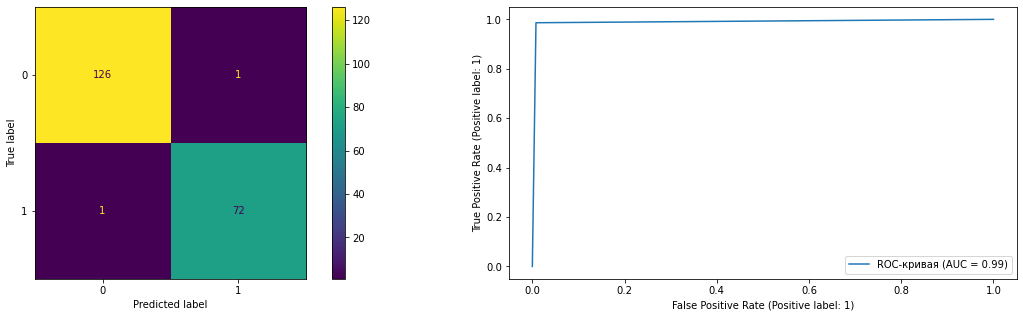
\includegraphics[width=\textwidth]{result}
\end{center}
\pagebreak

\subsubsection{sklearn.neighbors.KNeighborsClassifier}
\begin{alltt}
Лучшие гиперпараметры модели: {'knn__n_neighbors': 3}
Лучший счёт модели: 0.9950000000000001
Accuracy: 0.99
Recall: 0.9863013698630136
Precision: 0.9863013698630136
\end{alltt}
\begin{center}
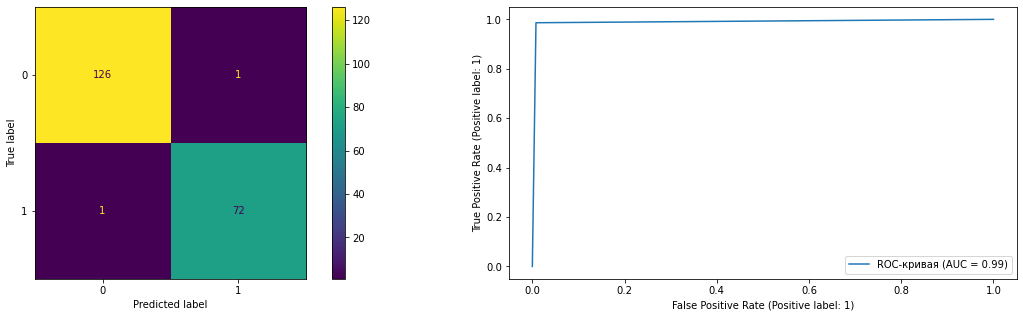
\includegraphics[width=\textwidth]{result}
\end{center}
\pagebreak

\subsection{Логистическая регрессия}
\subsubsection{LogisticRegression}
\begin{alltt}
Лучшие гиперпараметры модели: {'logreg__SGD_step': 0.05,
'logreg__batch_size': 5, 'logreg__epoches': 4}
Лучший счёт модели: 0.9950000000000001
Accuracy: 0.99
Recall: 0.9863013698630136
Precision: 0.9863013698630136
\end{alltt}
\begin{center}
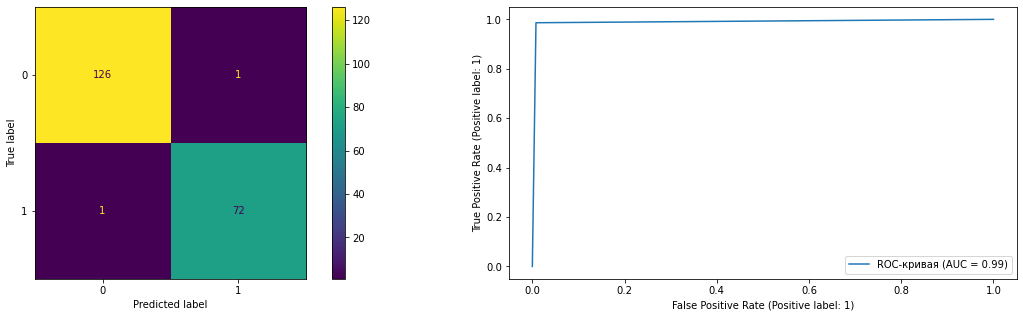
\includegraphics[width=\textwidth]{result}
\end{center}

\subsubsection{sklearn.linear\_model.LogisticRegression}
\begin{alltt}
Лучшие гиперпараметры модели: {'logreg__penalty': 'l2',
'logreg__solver': 'newton-cg'}
Лучший счёт модели: 0.9950000000000001
Accuracy: 0.99
Recall: 0.9863013698630136
Precision: 0.9863013698630136
\end{alltt}
\begin{center}
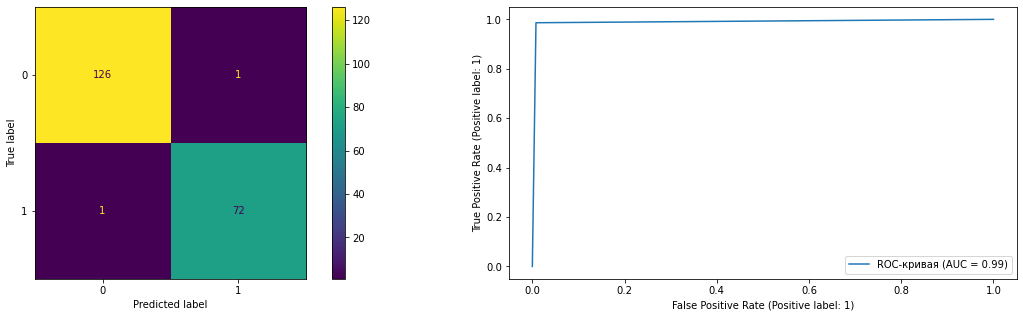
\includegraphics[width=\textwidth]{result}
\end{center}
\pagebreak

\subsection{Метод опорных векторов}
\subsubsection{SVM}
\begin{alltt}
Лучшие гиперпараметры модели: {'SVM__SGD_step': 0.01,
'SVM__alpha': 1.0, 'SVM__batch_size': 20, 'SVM__epoches': 4}
Лучший счёт модели: 0.9950000000000001
Accuracy: 0.99
Recall: 0.9863013698630136
Precision: 0.9863013698630136
\end{alltt}
\begin{center}
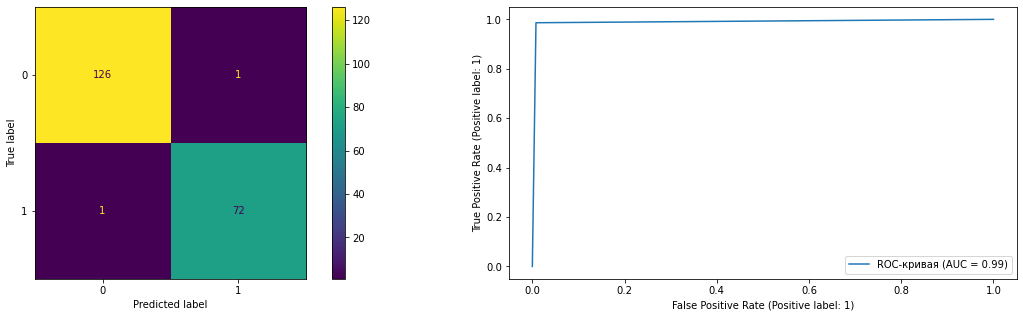
\includegraphics[width=\textwidth]{result}
\end{center}

\subsubsection{sklearn.svm.LinearSVC}
\begin{alltt}
Лучшие гиперпараметры модели: {'svc__loss': 'hinge', 'svc__max_iter': 10000.0}
Лучший счёт модели: 0.9950000000000001
Accuracy: 0.99
Recall: 0.9863013698630136
Precision: 0.9863013698630136
\end{alltt}
\begin{center}
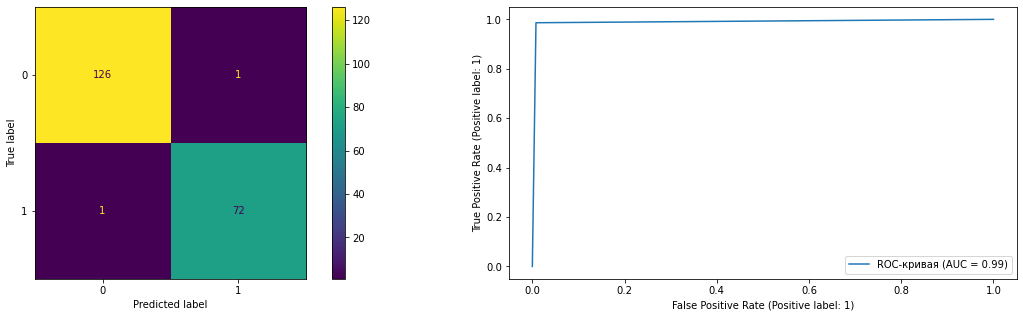
\includegraphics[width=\textwidth]{result}
\end{center}
\pagebreak

\subsection{Наивный байесовский классификатор}
\subsubsection{NaiveBayes}
\begin{alltt}
Accuracy: 0.99
Recall: 0.9863013698630136
Precision: 0.9863013698630136
\end{alltt}
\begin{center}
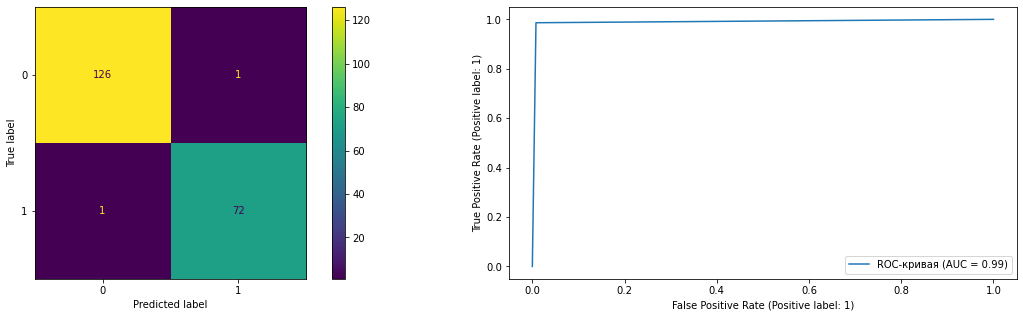
\includegraphics[width=\textwidth]{result}
\end{center}

\subsubsection{sklearn.naive\_bayes.GaussianNB}
\begin{alltt}
Accuracy: 0.99
Recall: 0.9863013698630136
Precision: 0.9863013698630136
\end{alltt}
\begin{center}
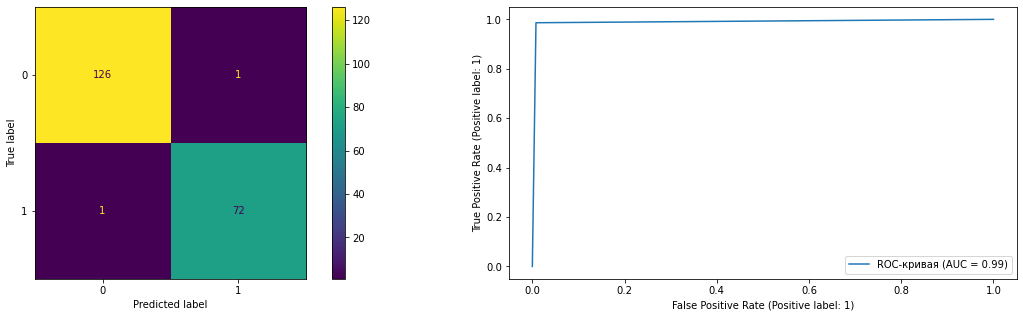
\includegraphics[width=\textwidth]{result}
\end{center}
\pagebreak

\subsection{Разделяющая прямая для метода опорных векторов}
\subsubsection{Моя реализация}
\begin{center}
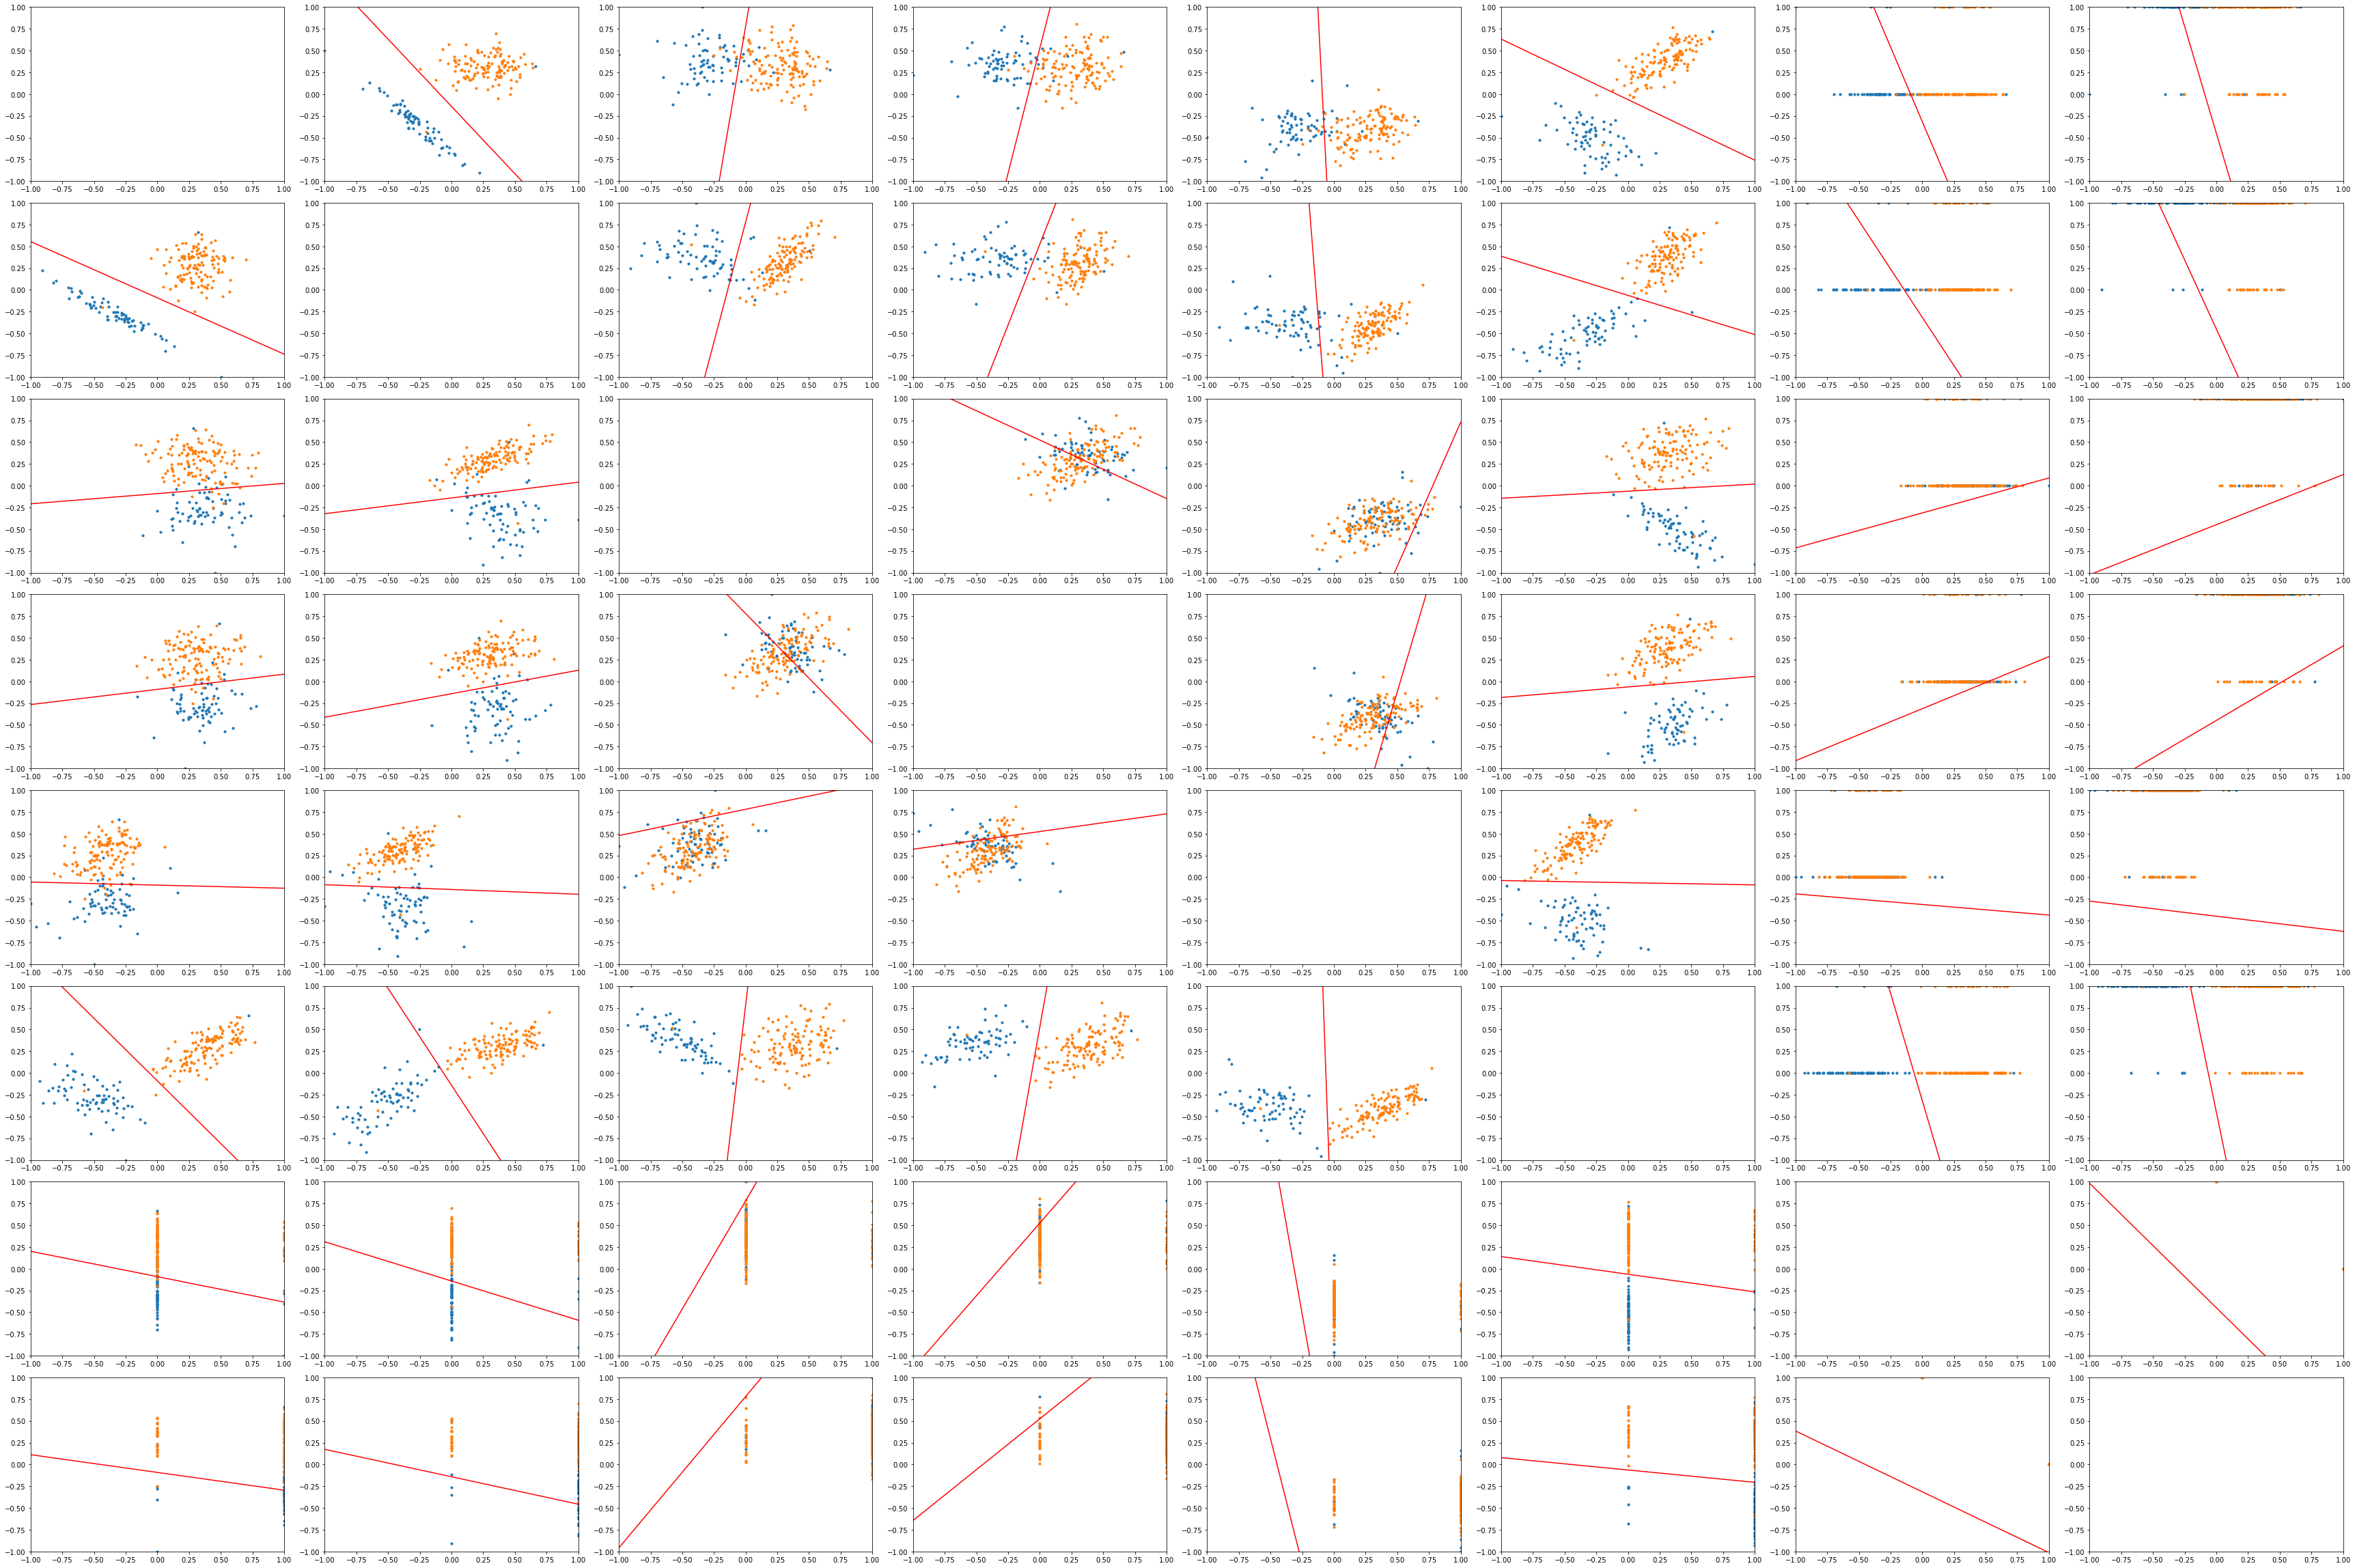
\includegraphics[width=\textwidth]{svm_lines_my}
\end{center}
\pagebreak

\subsubsection{sklearn.svm.LinearSVC}
\begin{center}
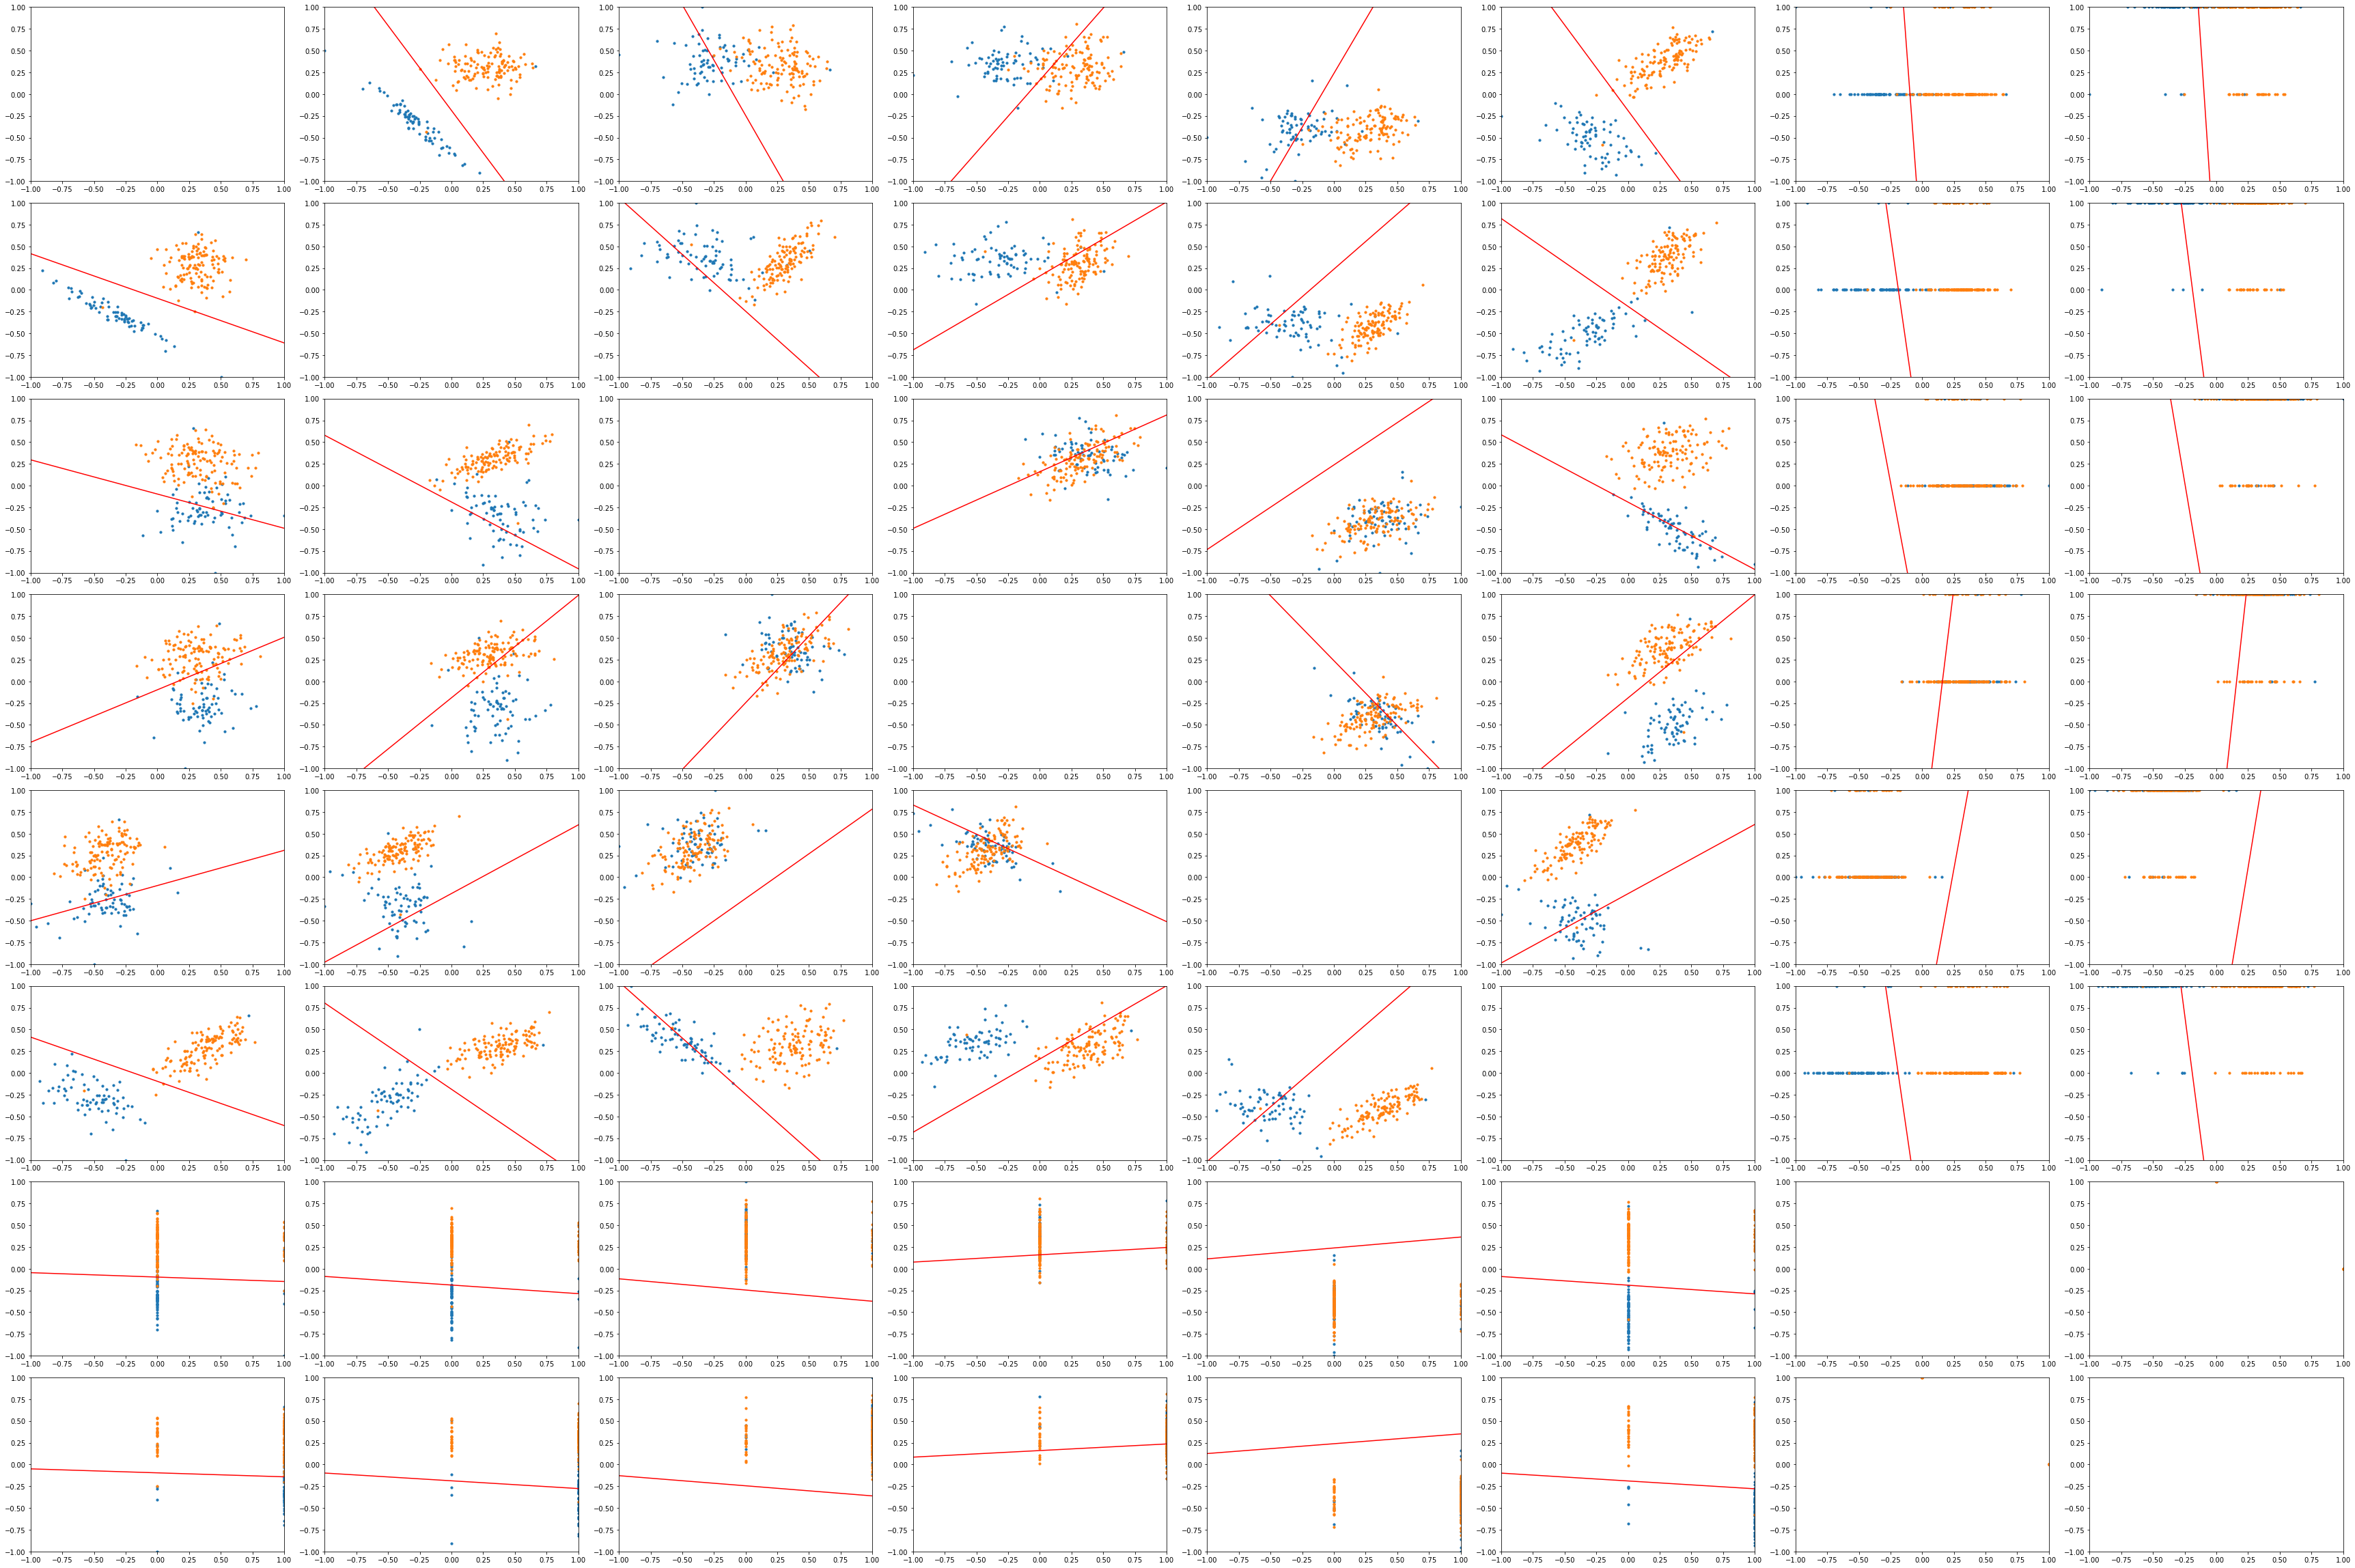
\includegraphics[width=\textwidth]{svm_lines}
\end{center}

\pagebreak
